%%%%%%%%%%%%%%%%%%%%%%%%%%%%%%%%%%%%%%%%%%
\section{Results}

\subsection{Forward Problem}\label{sec:results-forward}

\rev{Table~\ref{tab:forward} compares the methods on the three benchmarks of Section~\ref{sec:problem}. The Spectral-PINN appears in two versions. ``As submitted'' uses a soft Neumann penalty and 300 equispaced collocation points. ``Revised'' uses the exact Neumann basis and Gauss--Lobatto collocation. Errors are measured at $t=1$ ($t=5$ for B3) against the certified reference on the common 200-point grid. ``Mean~$\pm$~SD'' is over $n$ seeds. The table also gives $\max|u|$ over $x$ and $t$ and the number of energy increases on a time grid of spacing $0.02$.}

\begin{table}[H]
\caption{\rev{Forward problem on the three benchmarks. Errors against the certified reference on the common 200-point grid, mean $\pm$ SD over $n$ seeds; ``Energy incr.'' = number of increases of the energy over the intervals of a grid of spacing $0.02$ (total over seeds, $50T$ intervals per run); $\max|u|$ is the largest value over all runs of the row. Time is the training time of one run on an idle single core (rows with $^\dagger$: mean over the main runs, which were executed concurrently and are not a clean timing); the classical time is the median of three solves. The vanilla PINN has 8000 Adam epochs, the Spectral-PINN 6000 (+1000 warm-up) for $T=1$.}\label{tab:forward}}
\footnotesize
\begin{tabularx}{\textwidth}{Xccccccc}
\toprule
\textbf{Method} & \textbf{Params} & $L^2$ error & $L^\infty$ error & $n$ & Time (s) & $\max|u|$ & Energy incr.\\
\midrule
\multicolumn{8}{l}{\textit{B1: $\varepsilon=0.01$, $T=1$ (error at $t=1$)}}\\
Chebyshev collocation, $N=80$, $\delta t=0.0005$ & 81 & \ensuremath{5.37\times10^{-5}} & \ensuremath{6.48\times10^{-5}} & 1 & 0.21 & -- & --\\
Chebyshev collocation, $N=80$, $\delta t=0.0001$ & 81 & \ensuremath{1.07\times10^{-5}} & \ensuremath{1.30\times10^{-5}} & 1 & 1.29 & -- & --\\
Reaction-only ODE ($\varepsilon=0$) & 0 & \ensuremath{1.89\times10^{-3}} & \textbf{--} & 1 & -- & -- & --\\
Vanilla PINN & 8577 & \ensuremath{(6.86\pm1.59)\times10^{-2}} & \ensuremath{(9.80\pm2.18)\times10^{-2}} & 4 & 2081$^\dagger$ & 1.0084 & 0/200\\
Vanilla PINN + L-BFGS & 8577 & \textbf{--} & \textbf{--} & \textbf{--} & \textbf{--} & \textbf{--} & \textbf{--}\\
Spectral-PINN, as submitted, $K=32$ & 6433 & \textbf{--} & \textbf{--} & \textbf{--} & \textbf{--} & \textbf{--} & \textbf{--}\\
\quad + energy penalty ($\lambda_E=50$) & 6433 & \textbf{--} & \textbf{--} & \textbf{--} & \textbf{--} & \textbf{--} & \textbf{--}\\
Spectral-PINN, as submitted, $K=64$ & 8513 & \ensuremath{(9.93\pm1.56)\times10^{-2}} & \ensuremath{(1.71\pm0.30)\times10^{-1}} & 4 & 410$^\dagger$ & 1.0162 & 0/200\\
Spectral-PINN, revised, $K=32$ & 6303 & \ensuremath{(8.29\pm1.43)\times10^{-4}} & \ensuremath{(1.92\pm0.36)\times10^{-3}} & 5 & 251$^\dagger$ & 1.0013 & 0/250\\
\quad + energy penalty ($\lambda_E=50$) & 6303 & \ensuremath{(8.29\pm1.45)\times10^{-4}} & \ensuremath{(1.92\pm0.36)\times10^{-3}} & 5 & 214$^\dagger$ & 1.0013 & 0/250\\
\quad + L-BFGS & 6303 & \textbf{--} & \textbf{--} & \textbf{--} & \textbf{--} & \textbf{--} & \textbf{--}\\
Spectral-PINN, revised, $K=64$ & 8383 & \ensuremath{(1.46\pm0.42)\times10^{-3}} & \ensuremath{(3.66\pm0.92)\times10^{-3}} & 5 & 587$^\dagger$ & 1.0014 & 0/250\\
Spectral-PINN, revised, $K=128$ & 12543 & \ensuremath{(6.57\pm1.80)\times10^{-3}} & \ensuremath{(1.24\pm0.01)\times10^{-2}} & 2 & 732$^\dagger$ & 1.0014 & 0/100\\
\midrule
\multicolumn{8}{l}{\textit{B2: $\varepsilon=0.1$, $T=1$}}\\
Chebyshev collocation, $N=80$, $\delta t=0.0005$ & 81 & \ensuremath{5.10\times10^{-5}} & \ensuremath{6.95\times10^{-5}} & 1 & 0.21 & -- & --\\
Reaction-only ODE ($\varepsilon=0$) & 0 & \ensuremath{1.47\times10^{-1}} & \textbf{--} & 1 & -- & -- & --\\
Vanilla PINN & 8577 & \textbf{--} & \textbf{--} & \textbf{--} & \textbf{--} & \textbf{--} & \textbf{--}\\
Vanilla PINN + L-BFGS & 8577 & \textbf{--} & \textbf{--} & \textbf{--} & \textbf{--} & \textbf{--} & \textbf{--}\\
Spectral-PINN, as submitted, $K=32$ & 6433 & \textbf{--} & \textbf{--} & \textbf{--} & \textbf{--} & \textbf{--} & \textbf{--}\\
Spectral-PINN, revised, $K=32$ & 6303 & \textbf{--} & \textbf{--} & \textbf{--} & \textbf{--} & \textbf{--} & \textbf{--}\\
\quad + L-BFGS & 6303 & \textbf{--} & \textbf{--} & \textbf{--} & \textbf{--} & \textbf{--} & \textbf{--}\\
\midrule
\multicolumn{8}{l}{\textit{B3: $\varepsilon=0.05$, $T=5$ (error at $t=5$)}}\\
Chebyshev collocation, $N=96$, $\delta t=10^{-3}$ & 97 & \ensuremath{2.89\times10^{-5}} & \ensuremath{7.24\times10^{-5}} & 1 & 0.43 & -- & --\\
Reaction-only ODE ($\varepsilon=0$) & 0 & \ensuremath{4.64\times10^{-1}} & \textbf{--} & 1 & -- & -- & --\\
Vanilla PINN & 8577 & \textbf{--} & \textbf{--} & \textbf{--} & \textbf{--} & \textbf{--} & \textbf{--}\\
Spectral-PINN, revised, $K=32$ & 6303 & \textbf{--} & \textbf{--} & \textbf{--} & \textbf{--} & \textbf{--} & \textbf{--}\\
\quad + energy penalty & 6303 & \textbf{--} & \textbf{--} & \textbf{--} & \textbf{--} & \textbf{--} & \textbf{--}\\
Spectral-PINN, revised, $K=64$ & 8383 & \textbf{--} & \textbf{--} & \textbf{--} & \textbf{--} & \textbf{--} & \textbf{--}\\
\quad + energy penalty & 8383 & \textbf{--} & \textbf{--} & \textbf{--} & \textbf{--} & \textbf{--} & \textbf{--}\\
\bottomrule
\end{tabularx}

\end{table}


\rev{\emph{B1 ($\varepsilon=0.01$, $T=1$).} The revised Spectral-PINN ($K=32$) reaches a mean $L^2$ error of \mbox{\N{b1.fh_K32.l2}} over five seeds. The vanilla PINN reaches \N{b1.van.l2}. The ratio of seed means is \N{b1.ratio.van_fhK32}. The 95\% bootstrap interval is \N{b1.ratio.van_fhK32.ci}. The per-seed ratios are \N{b1.ratio.van_fhK32.range}. The ratio of maximum-norm errors is \N{b1.ratio.van_fhK32.linf}. This ratio replaces the two inconsistent values of the first version, 49 and 47. They were the ratio of five-seed means and the ratio for seed~42 alone. The seed-42 value used the original initial condition and the as-submitted network.}

\rev{An L-BFGS stage improves both PINNs. The vanilla PINN then reaches \N{b1.lb_van.l2}. The revised Spectral-PINN reaches \N{b1.lb_hard_K32.l2}. Both use three seeds. The ratio is \N{b1.ratio.lb}. The revised $K=32$ network is within a factor \N{b1.floor_ratio.K32} of the best polynomial of its degree. That least-squares floor is \N{floor.b1.K32.neumann} in the Neumann basis. The as-submitted network with $K=32$ is somewhat less accurate: \N{b1.so_K32.l2}, a factor \N{b1.ratio.so_fh_K32}. On B1 its soft penalty becomes harmful only for larger $K$ (Section~\ref{sec:results-k}). On B2 it is harmful already at $K=32$.}

\rev{\emph{The classical solver is the best method on B1.} Chebyshev collocation with $N=80$ and $\delta t=5\times10^{-4}$ reaches $L^2=\N{b1.cheb80.l2}$ in \N{b1.cheb80.time}~s. It is \N{b1.ratio.fh_K32_cheb80} times more accurate than the revised Spectral-PINN. It is about \N{b1.speed.fh_K32_cheb80} times faster. Time stepping dominates its error: $\delta t=10^{-4}$ gives \N{b1.cheb80.dt1e-4.l2}. B1 is also reaction-dominated. Solving $u'=u-u^3$ at each $x$ gives $L^2=\N{ode.compat.0.01.l2}$. So the revised Spectral-PINN is only \N{b1.ratio.ode_fh_K32} times closer to the solution than a model without diffusion. The vanilla PINN is further away than that model.}

\rev{\emph{B2 ($\varepsilon=0.1$, $T=1$).} Ignoring diffusion now gives $L^2=\N{ode.compat.0.1.l2}$. The revised Spectral-PINN reaches \N{b2.hard_K32.l2} (five seeds). That is \N{b2.ratio.ode_hard} times closer than the reaction-only model. The vanilla PINN reaches \N{b2.van.l2} (three seeds). The ratio is \N{b2.ratio.van_hard}. After an L-BFGS stage (one seed each) the order reverses. The vanilla PINN reaches \N{b2.lb_van.l2}. The revised Spectral-PINN reaches \N{b2.lb_hard_K32.l2}. So on B2 the coefficient network has no accuracy advantage over a well-trained space--time PINN. The weak boundary penalty of the as-submitted network hurts already at $K=32$. Its error is \N{b2.soft_K32.l2} (three seeds). Wall slopes reach \N{b2.soft.wall} and $\max|u|$ reaches \N{b2.soft.maxu}. The classical solver reaches \N{b2.cheb80.l2}.}

\rev{\emph{B3 ($\varepsilon=0.05$, $T=5$, sharp interfaces).} A polynomial of degree $32$ cannot represent the solution at $t=5$ better than $L^2\approx\N{floor.b3.K32}$ (least-squares floor on the evaluation grid). Degree $64$ can (\N{floor.b3.K64}). Neither network learns the dynamics. At $t=5$ the errors are \N{b3.K32_E0.l2} ($K=32$) and \N{b3.K64_E0.l2} ($K=64$, two seeds). These are as large as the solution itself. At $t=0.2$ they are already \N{b3.K32.t02} and \N{b3.K64.t02}. This is far above any representation limit. The training converged to a wrong trajectory. The energy penalty is active here, in \N{b3.E50.nz} epochs per run. It does not help: \N{b3.K64_E50.l2} for $K=64$. The vanilla PINN fails too (\N{b3.van.l2}). The classical solver reaches \N{b3.cheb.l2} ($N=80$, $\delta t=5\times10^{-4}$) and \N{b3.cheb128.l2} ($N=128$, $\delta t=10^{-4}$). Figure~\ref{fig:b3} shows the profiles.}

\begin{figure}[H]
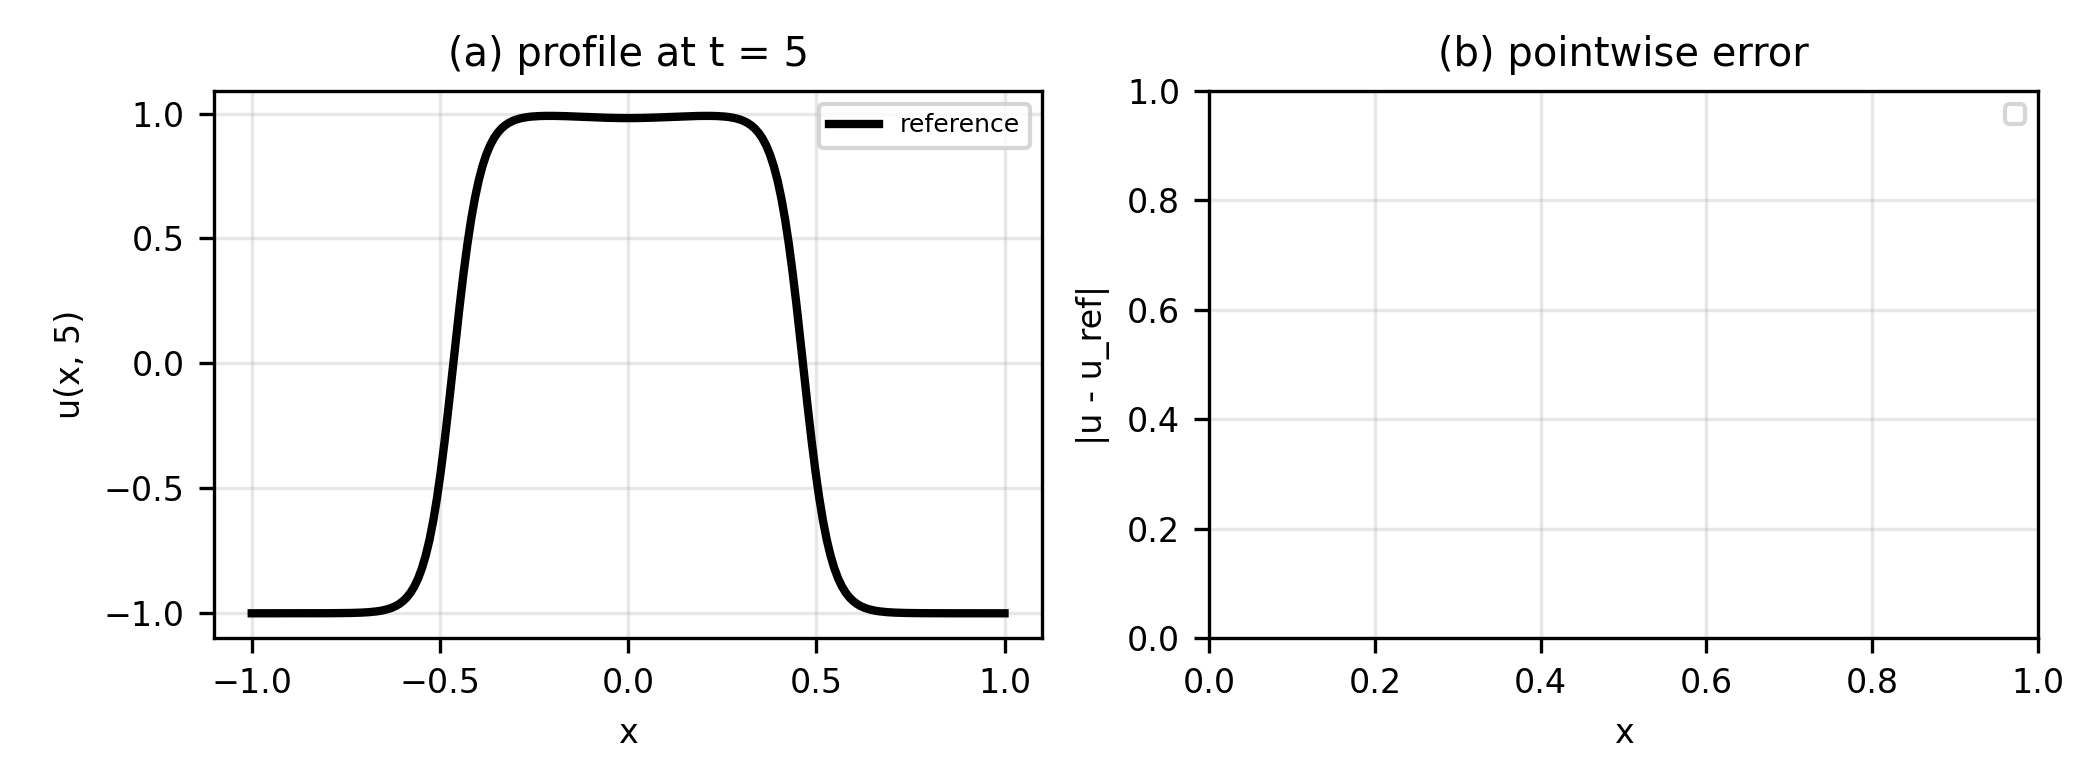
\includegraphics[width=\textwidth]{figures_r1/fig_b3.png}
\caption{\rev{B3 ($\varepsilon=0.05$, $T=5$, seed 42): certified reference and trained networks at $t=1$, $3$ and $5$.}\label{fig:b3}}
\end{figure}

\subsection{Mode Number and Boundary Penalty}\label{sec:results-k}

\rev{The first version reported that the accuracy of the Spectral-PINN \emph{degrades} as the number of modes $K$ grows. It blamed an optimization bottleneck of the coefficient parameterization. This was wrong. The cause was the boundary penalty. Its effective weight on $u_x(\pm1)^2$ was $\lambda_{\rm BC}K^{-4}$. It vanished as $K$ grew. The trained as-submitted $K=64$ networks have wall slopes $|u_x(\pm1)|$ up to \N{kk.soft64.wall} instead of zero. The $K=128$ network reaches \N{kk.soft128.wall} (Table~\ref{tab:K}).}

\rev{With the exact Neumann basis the $L^2$ error at $K=64$ is \N{kk.hard64.l2} (five seeds). The as-submitted variant gives \N{kk.soft64.l2}, a factor \N{kk.ratio_soft_hard64} worse. At $K=128$ the errors are \N{kk.hard128.l2} and \N{kk.soft128.l2} (Figure~\ref{fig:K}).}

\rev{Rescaling the soft penalty to unit weight ($\lambda_{\rm BC}=K^4$) does \emph{not} fix it. It makes it worse: \N{kk.fix64.l2} at $K=64$, with $\max|u|$ up to \N{kk.fix64.maxu}. The rescaled penalty $(\sum_kk^2c_k)^2$ has curvature of order $K^5/5$ in coefficient space. That is $2\times10^8$ at $K=64$, orders of magnitude above the other loss terms. With this conditioning the optimizer stops reducing the PDE residual. The time-RMS residual norm is \N{kk.fix64.rms}, against \N{kk.hard64.rms} for the exact basis. The wall slope is still \N{kk.fix64.wall}. A soft Neumann penalty thus fails at large $K$ in both directions. Scaled down with $K$, it is too weak. Not scaled, it is ill-conditioned. The exact basis removes the dilemma.}

\rev{The collocation grid has a secondary effect. Gauss--Lobatto instead of equispaced points improves the soft variant at $K=64$ by a factor \N{kk.cgl_soft_gain} (seed 42: \N{kk.soft_uniform64_s42} to \N{kk.soft_cgl64}). It stays far from the hard variant. With the exact basis the grid matters little (\N{kk.hard_uniform64} equispaced, \N{kk.hard_cgl64_s42} Gauss--Lobatto, seed 42).}

\rev{With the revised variant and the default budget, a smaller trend remains. The error grows from \N{kk.hard32.l2} at $K=32$ by a factor \N{kk.ratio64_32} at $K=64$. It grows by a further factor \N{kk.ratio128_64} at $K=128$. This is an optimization effect, not a representation limit. The best polynomials of degree 64 and 128 approximate the solution to \N{floor.b1.K64} and \N{floor.b1.K128}. More budget helps. Doubling the epochs lowers the $K=64$ error of seed 42 from \N{kk.hard_cgl64_s42} to \N{kk.kh_K64_x2.l2}. This is below the floor of $K=32$ (\N{floor.b1.K32.neumann}). An L-BFGS stage after Adam gives \N{b1.lb_hard_K64.l2} (two seeds). At $K=128$ twice the budget gives \N{kk.kh_K128_x2.l2} (default: \N{kk.hard128_s42}). At $K=256$ the default budget gives \N{kk.kh_K256_x1.l2} (seed 42). The as-submitted network gave $1.5$ in the first version. A larger $K$ needs a larger budget. The errors of order one do not occur.}

\begin{table}[H]
\caption{\rev{Effect of the mode number $K$ for different treatments of the Neumann condition and of the collocation grid (B1, $L^2$ error at $t=1$). Budget is the number of epochs relative to $6000+1000$ warm-up epochs. Single-seed rows have $n=1$ (SD not defined). The wall slope is the maximum of $|u_x(\pm1,t)|$ over the trained trajectory. Times marked $^\dagger$ come from concurrently executed runs.}\label{tab:K}}
\small
\begin{tabularx}{\textwidth}{p{4.8cm}cccccc}
\toprule
\textbf{Variant} & $K$ & Budget & $L^2$ error & max $|u_x(\pm1)|$ & $n$ & Time (s)\\
\midrule
soft penalty, equispaced grid (as submitted) & 32 & $1\times$ & \textbf{--} & \textbf{--} & 0 & \textbf{--}\\
 & 64 & $1\times$ & \ensuremath{(9.93\pm1.56)\times10^{-2}} & 5.67 & 4 & 410$^\dagger$\\
 & 128 & $1\times$ & \textbf{--} & \textbf{--} & 0 & \textbf{--}\\
soft penalty, Gauss--Lobatto grid & 32 & $1\times$ & \ensuremath{9.33\times10^{-4}} & 0.55 & 1 & 192$^\dagger$\\
 & 64 & $1\times$ & \ensuremath{1.52\times10^{-2}} & 4.02 & 1 & 446$^\dagger$\\
soft penalty rescaled ($\lambda_{\rm BC}=K^4$) & 32 & $1\times$ & \textbf{--} & \textbf{--} & 0 & \textbf{--}\\
 & 64 & $1\times$ & \textbf{--} & \textbf{--} & 0 & \textbf{--}\\
 & 128 & $1\times$ & \textbf{--} & \textbf{--} & 0 & \textbf{--}\\
\midrule
exact Neumann basis, equispaced grid & 64 & $1\times$ & \ensuremath{2.07\times10^{-3}} & 0.00 & 1 & 475$^\dagger$\\
exact Neumann basis, Gauss--Lobatto grid (revised) & 32 & $1\times$ & \ensuremath{(8.29\pm1.43)\times10^{-4}} & 0.00 & 5 & 251$^\dagger$\\
 & 64 & $1\times$ & \ensuremath{(1.46\pm0.42)\times10^{-3}} & 0.00 & 5 & 587$^\dagger$\\
 & 128 & $1\times$ & \ensuremath{(6.57\pm1.80)\times10^{-3}} & 0.00 & 2 & 732$^\dagger$\\
 & 64 & $2\times$ & \textbf{--} & \textbf{--} & 0 & \textbf{--}\\
 & 128 & $2\times$ & \textbf{--} & \textbf{--} & 0 & \textbf{--}\\
 & 256 & $1\times$ & \textbf{--} & \textbf{--} & 0 & \textbf{--}\\
\bottomrule
\end{tabularx}

\end{table}


\begin{figure}[H]
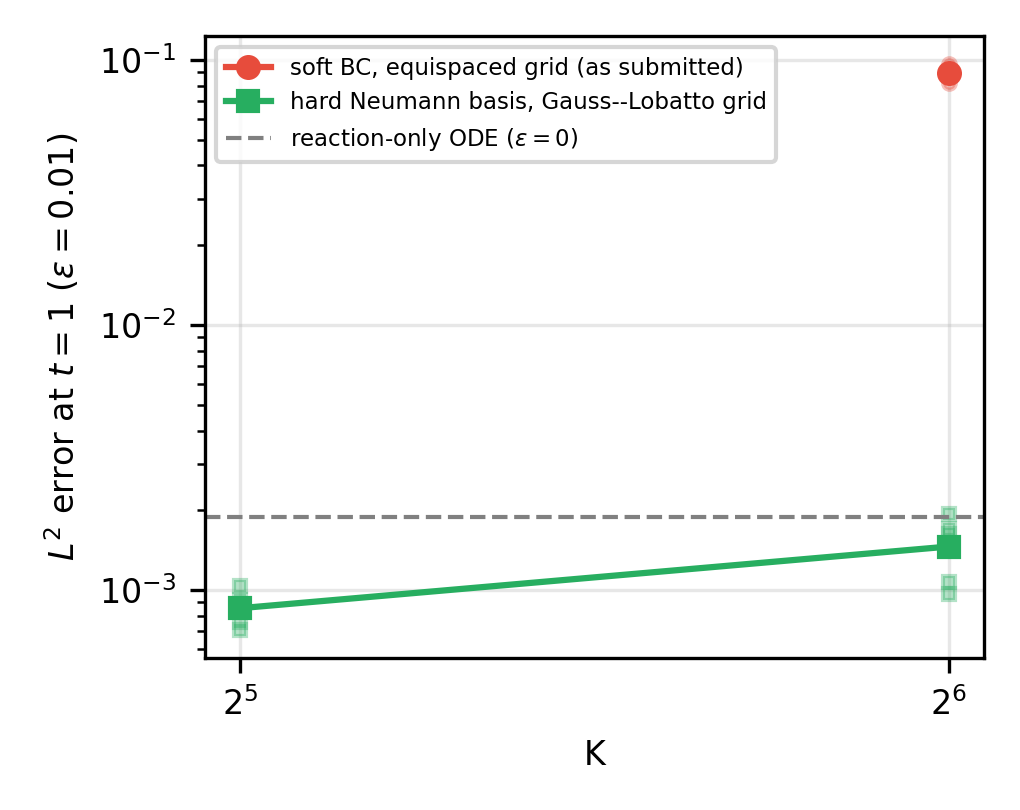
\includegraphics[width=8.5cm]{figures_r1/fig_K.png}
\caption{\rev{$L^2$ error at $t=1$ versus the mode number $K$ (B1; small symbols: individual seeds, large: mean). Curves: as-submitted soft penalty with effective weight $K^{-4}$; the same penalty rescaled to unit weight ($\lambda_{\rm BC}=K^4$); the revised Spectral-PINN at the default and at twice the default budget. The dashed line is the error of the reaction-only model.}\label{fig:K}}
\end{figure}

\subsection{Energy Penalty}\label{sec:results-energy}

\rev{The first version used $\lambda_E=50$ in all penalized runs but did not report it.}

\subsubsection{Energy Decreases in Every Run}

\rev{In B1 we trained \N{en.n_runs} Spectral-PINNs, with and without the penalty. They include the inaccurate networks of Section~\ref{sec:results-k} (errors up to \N{en.max_l2}) and the poor-trajectory regimes below. Every one decreases its energy on every interval of the grids with spacing $0.02$, $0.002$ and $2\times10^{-4}$. The vanilla PINNs of B1 (grid $0.02$ only) have \N{en.van_viol} increases in \N{mbp.n_van} runs.}

\subsubsection{The Penalty Is Inactive}

\rev{For the revised $K=32$ network the energy drops by at least \N{en.min_step} per interval of length $0.02$. The penalty changes the energy trajectory by at most \N{en.max_diff}, comparing the same seed with and without it. So the two curves of Figure~\ref{fig:energy}(a) coincide. The zero violations of the first version cannot be attributed to the penalty. The penalty term is positive in \N{en.nonzero} training epochs of the five runs with $\lambda_E=50$. Table~\ref{tab:energy} varies $\lambda_E$ from $0$ to $5000$. The mean error stays between \N{en.lam.min} and \N{en.lam.max} for all six weights. The seed-to-seed SD at $\lambda_E=0$ is \N{en.lam.sd}. No network has an energy increase. The penalty is nonzero in at most \N{en.lam.max_nonzero} epoch per run. Its largest weighted value is \N{en.lam.maxpen}, at $\lambda_E=5000$.}

\subsubsection{Poor-Trajectory Regimes}

\rev{We looked for regimes where the trajectory is poor. They are: a run cut to \N{reg.short_epochs} epochs, no warm-up, a ten times smaller learning rate with 1500 epochs, and $K=64$ with the as-submitted soft penalty (Table~\ref{tab:energy}, lower part). The truncated and slow runs have large errors (\N{reg.short.E0} and \N{reg.pde0.E0}). Their energy is still monotone without the penalty. The penalty is active in at most \N{reg.pde0.E50.maxnz} epochs per run. The errors with it (\N{reg.short.E50}, \N{reg.pde0.E50}) agree with those without it. For the as-submitted $K=64$ network the penalty is active in \N{reg.soft64.nz} epochs per run. It changes the error by less than the seed-to-seed scatter: \N{reg.soft64.E50} against \N{reg.soft64.E0} for the same seeds. It is slightly lower with the penalty for each of the three seeds.}

\subsubsection{Training Without Warm-Up}

\rev{The only regime with a substantial effect is training without warm-up. The untrained initial trajectory has increasing energy. The penalty is active in up to \N{reg.nowarm.E50.maxnz} epochs per run, with weighted values up to \N{reg.nowarm.E50.maxpen}. The result is \emph{worse}: \N{reg.nowarm.E50} against \N{reg.nowarm.E0} without the penalty. The error is larger for all three seeds, by factors of \N{reg.nowarm.factors}. In none of the \N{reg.n_runs} runs of these regimes does the final network have an energy increase. Monotone energy is thus not a diagnostic of accuracy here. Networks with errors of order one satisfy it.}

\begin{table}[H]
\caption{\rev{Energy penalty weight and regime (revised Spectral-PINN, $K=32$, B1). ``increases'' is the total number of energy increases (more than $10^{-10}$) over all seeds on grids of spacing $0.02$, $0.002$, $2\times10^{-4}$; ``penalty $>0$'' is the largest number, over the seeds, of training epochs at which $\mathcal L_E>0$ (out of the total number of epochs).}\label{tab:energy}}
\small
\begin{tabularx}{\textwidth}{p{4.6cm}cccc}
\toprule
Setting & $n$ & $L^2$ error at $t=1$ & increases (0.02 / 0.002 / $2\times10^{-4}$) & penalty $>0$ in epochs\\
\midrule
$\lambda_E=0$ & 5 & \ensuremath{(8.29\pm1.43)\times10^{-4}} & 0 / 0 / 0 & 0\\
$\lambda_E=1$ & 0 & \textbf{--} & \textbf{--} & \textbf{--}\\
$\lambda_E=10$ & 0 & \textbf{--} & \textbf{--} & \textbf{--}\\
$\lambda_E=50$ & 5 & \ensuremath{(8.29\pm1.45)\times10^{-4}} & 0 / 0 / 0 & 1\\
$\lambda_E=500$ & 0 & \textbf{--} & \textbf{--} & \textbf{--}\\
$\lambda_E=5000$ & 0 & \textbf{--} & \textbf{--} & \textbf{--}\\
\midrule
300 epochs, warm-up 100, $\lambda_E=0$ & 0 & \textbf{--} & \textbf{--} & \textbf{--}\\
300 epochs, warm-up 100, $\lambda_E=50$ & 0 & \textbf{--} & \textbf{--} & \textbf{--}\\
no warm-up, $\lambda_E=0$ & 0 & \textbf{--} & \textbf{--} & \textbf{--}\\
no warm-up, $\lambda_E=50$ & 0 & \textbf{--} & \textbf{--} & \textbf{--}\\
learning rate $10^{-4}$, 1500 epochs, $\lambda_E=0$ & 0 & \textbf{--} & \textbf{--} & \textbf{--}\\
learning rate $10^{-4}$, 1500 epochs, $\lambda_E=50$ & 0 & \textbf{--} & \textbf{--} & \textbf{--}\\
\bottomrule
\end{tabularx}

\end{table}


\begin{figure}[H]
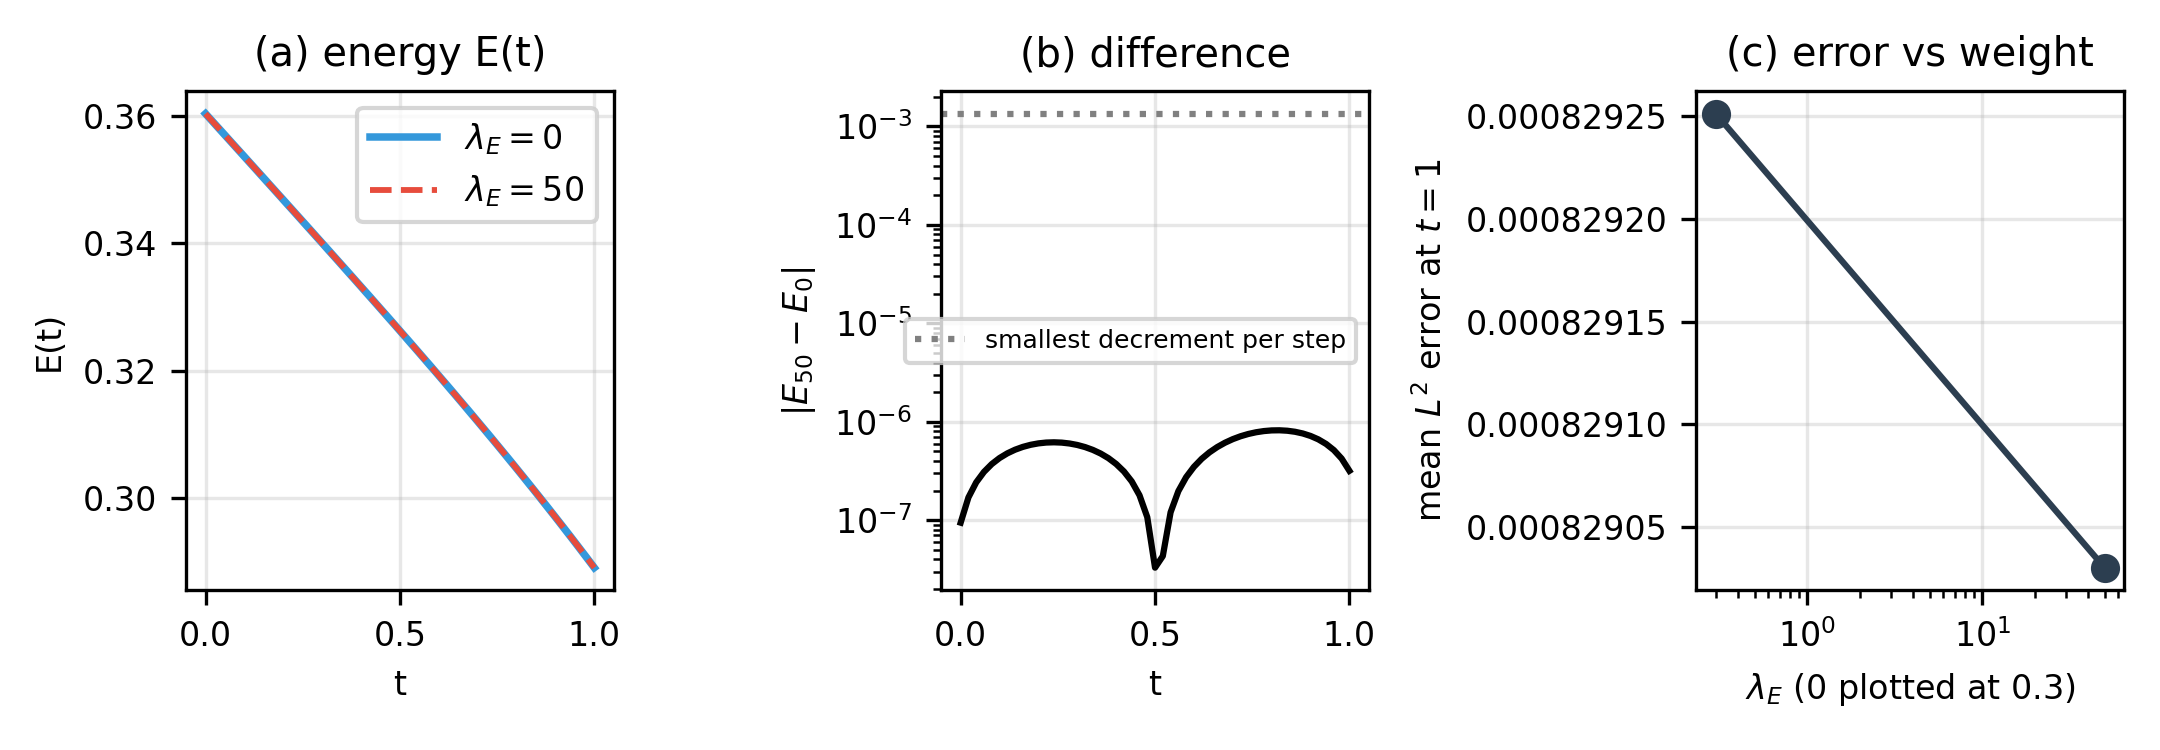
\includegraphics[width=\textwidth]{figures_r1/fig_energy.png}
\caption{\rev{Energy of the trained trajectory (B1, revised $K=32$, seed 42) with and without the energy penalty. (a)~$E(t)$. (b)~Absolute difference of the two curves, compared with the smallest decrement of $E$ per grid interval. (c)~Mean $L^2$ error versus $\lambda_E$ (five seeds).}\label{fig:energy}}
\end{figure}

\subsection{Maximum Bound and Energy Balance}\label{sec:results-balance}

\rev{\emph{Maximum bound.} The exact solution satisfies $|u|\le1$. The certified reference of B1 has $\max|u|=\N{mbp.ref_max_t1}$ at $t=1$. Decreasing energy does not imply the bound~\cite{ref_Du2021b,ref_He2019}. We computed $\max_{x,t}|u_\theta|$ for every one-dimensional network trained on the forward problem. Table~\ref{tab:forward} gives the largest value per configuration.}

\rev{All \N{mbp.n_hard} revised Spectral-PINNs of B1 outside the poor-trajectory regimes exceed the bound slightly. The excess is at most \N{mbp.excess} (largest value \N{mbp.max_hard}). The \N{mbp.n_hard_reg} revised networks of the poor-trajectory regimes exceed it by up to \N{mbp.excess_reg} (largest value \N{mbp.max_hard_reg}). Also \N{mbp.n_van_over} of the \N{mbp.n_van} vanilla PINNs of B1 exceed it, by up to \N{mbp.van_excess}. These excesses are of the order of the approximation error. But the bound is \emph{not} guaranteed. The inaccurate networks of Section~\ref{sec:results-k} violate it substantially. $\max|u|$ reaches \N{kk.fix64.maxu} for the rescaled soft penalty and \N{kk.soft128.maxu} for the as-submitted network with $K=128$. Their energy still decreases monotonically. A guaranteed bound would need an extra mechanism such as a limiter~\cite{ref_Geng2025}. We do not attempt one.}

\rev{\emph{Energy balance.} For every Spectral-PINN trained for the forward problem we evaluated both sides of the identity~\eqref{eq:balance-main} and the bound~\eqref{eq:balance-int} (Table~\ref{tab:balance}). The identity holds to round-off. The largest relative deviation is \N{bal.id_err} over all \N{bal.n} networks. This checks the code against Theorem~\ref{thm:balance}.}

\rev{For the revised $K=32$ networks (B1), the time-integrated residual $\frac12\int_0^T\|r\|^2\,dt$ is \N{bal.int_r_hard} on average and at most \N{bal.int_r_hard_max} over the five seeds. The energy decrease is $E(0)-E(T)=\N{bal.dE_hard}$. So no such network can gain more than \N{bal.int_r_hard_max} of energy between any two times. This is a fraction \N{bal.frac_hard_max} of the decrease. The decay is driven by $\|u_t\|^2$, not by the residual. For the as-submitted soft variant at $K=64$ the residual term is \N{bal.int_r_soft64}. The boundary defect adds \N{bal.int_b_soft}. Figure~\ref{fig:balance}(a) compares both sides of the identity along a trained trajectory. Figure~\ref{fig:balance}(b) shows the residual of trained networks.}

\begin{table}[H]
\caption{\rev{A-posteriori energy balance of the trained trajectories (Section~\ref{sec:balance}): wall slope, time-integrated residual $\frac12\int_0^T\|r\|^2dt$, time-integrated boundary defect, actual energy decrease, and relative error of the identity~\eqref{eq:balance-main} checked against the autograd derivative of $E(t)$ (maximum over seeds). Means over seeds.}\label{tab:balance}}
\small
\begin{tabularx}{\textwidth}{Xcccccc}
\toprule
\textbf{Network} & $n$ & max $|u_x(\pm1)|$ & $\frac12\!\int\!\|r\|^2$ & $\int|\beta|$ & $E(0)-E(T)$ & id. error\\
\midrule
revised $K=32$ & 5 & 3.6e-15 & \ensuremath{1.28\times10^{-5}} & \ensuremath{3.72\times10^{-22}} & 0.071 & \ensuremath{3.4\times10^{-16}}\\
revised $K=32$, $\lambda_E=50$ & 5 & 3.6e-15 & \ensuremath{1.28\times10^{-5}} & \ensuremath{4.12\times10^{-22}} & 0.071 & \ensuremath{3.4\times10^{-16}}\\
revised $K=64$ & 5 & 4.4e-15 & \ensuremath{2.08\times10^{-5}} & \ensuremath{4.01\times10^{-22}} & 0.071 & \ensuremath{3.4\times10^{-16}}\\
revised $K=128$ & 2 & 7.1e-15 & \ensuremath{5.86\times10^{-5}} & \ensuremath{1.94\times10^{-21}} & 0.070 & \ensuremath{3.4\times10^{-16}}\\
as submitted $K=64$ & 4 & 5.7e+00 & \ensuremath{4.57\times10^{-4}} & \ensuremath{4.11\times10^{-6}} & 0.058 & \ensuremath{4.4\times10^{-16}}\\
revised, B2 & 0 & \textbf{--} & \textbf{--} & \textbf{--} & \textbf{--} & \textbf{--}\\
revised $K=64$, B3 & 0 & \textbf{--} & \textbf{--} & \textbf{--} & \textbf{--} & \textbf{--}\\
\bottomrule
\end{tabularx}

\end{table}


\begin{figure}[H]
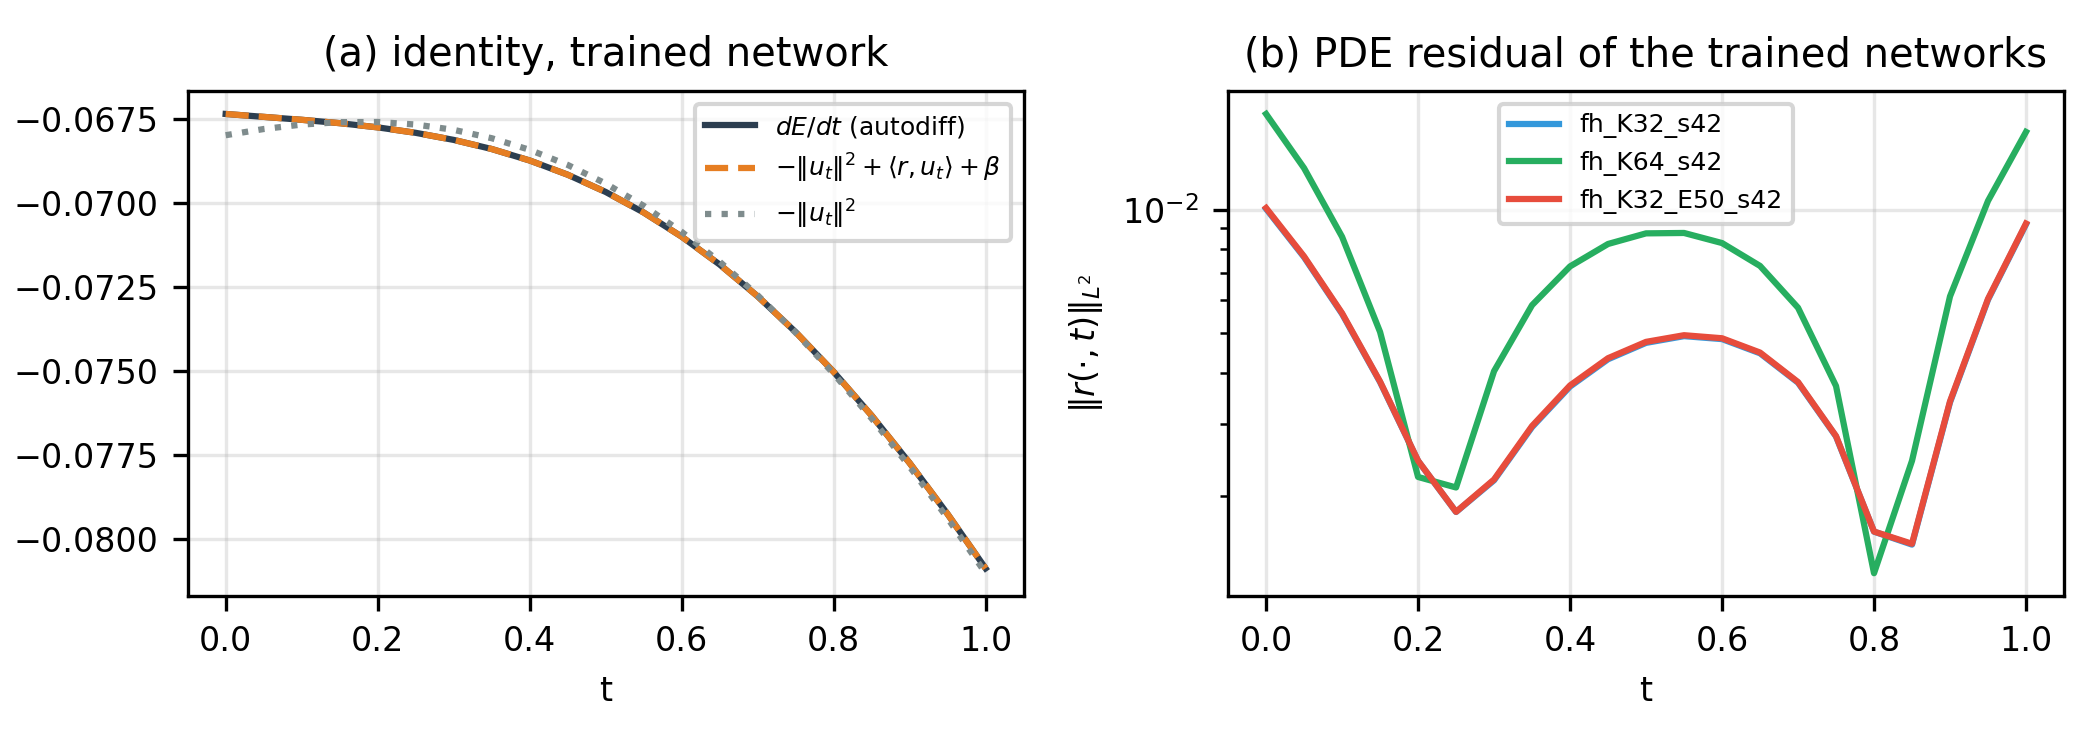
\includegraphics[width=\textwidth]{figures_r1/fig_balance.png}
\caption{\rev{(a) The two sides of the energy identity~\eqref{eq:balance-main} along the trained trajectory (B1, revised $K=32$, $\lambda_E=50$, seed 42). They coincide to round-off. (b) $L^2$ norm of the PDE residual versus time. Curves: revised $K=32$ without ($\lambda_E=0$, solid) and with ($\lambda_E=50$, dashed) the energy penalty, which nearly coincide, and revised $K=64$ (B1, seed 42).}\label{fig:balance}}
\end{figure}

\subsection{Inverse Problem}\label{sec:results-inverse}

\subsubsection{Joint Adam Depends on the Starting Value}

\rev{The first version reported a ``robust $\sim38\%$ overestimation bias'' of $\varepsilon$. It blamed the loss weighting, the warm-up or the observation design, without an ablation. The bias is the footprint of the starting value and of the optimizer.}

\rev{With joint Adam (Section~\ref{sec:inverse}) the recovered value is $\hat\varepsilon\approx\N{inv.ratio_mean}\,\varepsilon_{\rm init}$. The range is \N{inv.ratio_range} over \N{inv.n_sweep} runs. This holds for every $\varepsilon_{\rm init}\in\{0.5,1,1.5,2,4\}\,\varepsilon_{\rm true}$, for $\varepsilon_{\rm true}\in\{0.05,0.1\}$ and for both the as-submitted and the revised network (Figure~\ref{fig:inverse}(a), Table~\ref{tab:inverse1}). All runs of the first version that gave $38\%$ started from $\varepsilon_{\rm init}=2\varepsilon_{\rm true}$. And $0.7\times2=1.4$ is the ``bias''.}

\rev{Most of the displacement of $\log\varepsilon$ happens at the start of the joint phase. The median is \N{inv.frac200} of the total within the first 200 of 4000 epochs. The minimum is \N{inv.frac200_min}. The learning rate of $\log\varepsilon$ sets its size. The displacement $|\log(\hat\varepsilon/\varepsilon_{\rm init})|$ is \N{inv.ab.mult1.disp}, \N{inv.ab.base.disp} and \N{inv.ab.mult100.disp} for multipliers $1$, $10$ (default) and $100$ (Table~\ref{tab:inverse2}).}

\rev{The data enter only weakly. The estimate lies in the range \N{inv.ab.design_range}$\,\varepsilon_{\rm true}$ for 10, 40 or 160 observation points, 5 or 20 observation times, $K=16$, $32$ or $64$ and $\lambda_{\rm PDE}=5$, $50$ or $500$. A thousand times larger data weight moves it to \N{inv.ab.ld2000.rt}$\,\varepsilon_{\rm true}$. Four times more epochs move it to \N{inv.ab.ep16000.rt}$\,\varepsilon_{\rm true}$. Started from the true value, the estimate first moves away from it, to about $0.7\,\varepsilon_{\rm true}$ within 200 epochs. With the large data weight the data pull it back to \N{inv.ab.ld2000_i1.rt}$\,\varepsilon_{\rm true}$. With the default weight it ends at \N{inv.i1.rt}$\,\varepsilon_{\rm true}$.}

\rev{The first version also reported noise experiments at $\varepsilon_{\rm true}=0.01$ ($40.2$, $40.2$ and $40.0\%$ for $\sigma=0$, $0.01$ and $0.05$) and one run at $\varepsilon_{\rm true}=0.05$ ($14.7\%$). They came from a script whose settings differed from those stated. Its output was not archived. We withdraw these numbers.}

\subsubsection{Variable Projection}

\rev{Variable projection (Section~\ref{sec:inverse}) uses a data-fitting phase and a large data weight. On noise-free data it recovers $\varepsilon$ with relative errors of \N{inv.vp_err_005} ($\varepsilon_{\rm true}=0.05$) and \N{inv.vp_err_01} ($0.1$) at $\lambda_{\rm data}=2000$ (Figure~\ref{fig:inverse}(b), Table~\ref{tab:inverse2}). It needs a large data weight and enough observation points. With $\lambda_{\rm data}=20$ the errors are \N{inv.vp.e0.05.ld20} and \N{inv.vp.e0.1.ld20}. With only 10 observation points the error is \N{inv.vp.nx10}. With $K=64$ the least-squares value of $\varepsilon^2$ collapsed to its lower bound $10^{-8}$ during training.}

\subsubsection{Robustness to Noise}

\rev{The estimator is not robust to noise (Table~\ref{tab:inverse3}, Figure~\ref{fig:inverse}(c)). With $\sigma=0.01$ it underestimates $\varepsilon$ by \N{inv.vpn.e0.05.n0.01} ($\varepsilon_{\rm true}=0.05$) and \N{inv.vpn.e0.1.n0.01} ($0.1$), averaged over five noise realizations. With $\sigma=0.05$ it collapses toward $\varepsilon=0$. The largest estimate is \N{inv.vpn.e0.1.n0.05.maxratio}$\,\varepsilon_{\rm true}$. A plausible cause, not investigated further: with a large data weight the network fits part of the noise. This raises $\|u_{xx}\|$ and lowers the least-squares value.}

\rev{Classical least squares (Section~\ref{sec:inverse}) does better on the same realizations. Its mean errors are \N{inv.cl5.e0.05.n0.01} and \N{inv.cl5.e0.1.n0.01} for $\sigma=0.01$. They are \N{inv.cl5.e0.05.n0.05} and \N{inv.cl5.e0.1.n0.05} for $\sigma=0.05$. This agrees with the Cram\'er--Rao bound. Without noise it recovers the true value to better than $10^{-3}\%$, because the data come from the same solver.}

% generated by make_tex_r1.py -- do not edit
\begin{table}[H]
\tablesize{\footnotesize}
\caption{Joint Adam (procedure of the first version). Estimate $\hat\varepsilon/\varepsilon_{\rm true}$ for five starting values. Noise-free data, seed 42. Last row: $\hat\varepsilon/\varepsilon_{\rm init}$, mean~$\pm$~SD over the five starting values.\label{tab:inverse1}}
\newcolumntype{C}{>{\centering\arraybackslash}X}
\begin{tabularx}{\textwidth}{cCCCC}
\toprule
\ensuremath{\boldsymbol{\varepsilon_{\rm init}/\varepsilon_{\rm true}}} & \multicolumn{2}{c}{$\boldsymbol{\varepsilon_{\rm true}=0.05}$} & \multicolumn{2}{c}{$\boldsymbol{\varepsilon_{\rm true}=0.1}$}\\
 & \textbf{as submitted} & \textbf{revised} & \textbf{as submitted} & \textbf{revised}\\
\midrule
0.50 & 0.361 & 0.307 & 0.357 & 0.342\\
1.0 & 0.713 & 0.679 & 0.717 & 0.685\\
1.5 & 1.08 & 1.10 & 1.08 & 1.01\\
2.0 & 1.43 & 1.37 & 1.43 & 1.37\\
4.0 & 2.87 & 2.73 & 2.87 & 2.81\\
\midrule
$\hat\varepsilon/\varepsilon_{\rm init}$ & \ensuremath{0.717\pm0.003} & \ensuremath{0.678\pm0.043} & \ensuremath{0.716\pm0.002} & \ensuremath{0.685\pm0.011}\\
\bottomrule
\end{tabularx}
\end{table}

\begin{table}[H]
\tablesize{\footnotesize}
\caption{Inverse problem, noise-free data. Sensitivity of the joint-Adam and variable-projection estimates to the settings. One run each, seed 42.\label{tab:inverse2}}
\newcolumntype{C}{>{\centering\arraybackslash}X}
\begin{tabularx}{\textwidth}{Xcccc}
\toprule
\textbf{Setting} & \ensuremath{\boldsymbol{\varepsilon_{\rm true}}} & \ensuremath{\boldsymbol{\hat\varepsilon/\varepsilon_{\rm true}}} & \ensuremath{\boldsymbol{\hat\varepsilon/\varepsilon_{\rm init}}} & \textbf{Data RMS misfit}\\
\midrule
\multicolumn{5}{l}{\emph{Joint Adam, revised network, $\varepsilon_{\rm init}=2\varepsilon_{\rm true}$}}\\
default ($\lambda_{\rm data}=2$, 40 points, 5 times, $K=32$) & 0.05 & 1.37 & 0.685 & \ensuremath{1.4\times10^{-2}}\\
$\lambda_{\rm data}=2000$ & 0.05 & 1.14 & 0.572 & \ensuremath{1.5\times10^{-3}}\\
$\lambda_{\rm data}=2000$, $\varepsilon_{\rm init}=\varepsilon_{\rm true}$ & 0.05 & 1.02 & 1.02 & \ensuremath{1.1\times10^{-3}}\\
10 observation points & 0.05 & 1.36 & 0.681 & \ensuremath{1.5\times10^{-2}}\\
160 observation points & 0.05 & 1.37 & 0.684 & \ensuremath{1.4\times10^{-2}}\\
20 observation times & 0.05 & 1.32 & 0.661 & \ensuremath{1.4\times10^{-2}}\\
$K=16$ & 0.05 & 1.32 & 0.662 & \ensuremath{1.2\times10^{-2}}\\
$K=64$ & 0.05 & 1.29 & 0.647 & \ensuremath{1.1\times10^{-2}}\\
$\lambda_{\rm PDE}=5$ & 0.05 & 1.30 & 0.652 & \ensuremath{5.6\times10^{-3}}\\
$\lambda_{\rm PDE}=500$ & 0.05 & 1.30 & 0.648 & \ensuremath{6.9\times10^{-2}}\\
learning-rate multiplier of $\log\varepsilon$: 1 (default 10) & 0.05 & 1.81 & 0.907 & \ensuremath{2.1\times10^{-2}}\\
learning-rate multiplier of $\log\varepsilon$: 100 & 0.05 & 0.168 & 0.0842 & \ensuremath{1.1\times10^{-2}}\\
16\,000 epochs (default 4000) & 0.05 & 0.705 & 0.352 & \ensuremath{4.0\times10^{-3}}\\
\midrule
\multicolumn{5}{l}{\emph{Variable projection (data-fit phase of 3000 epochs, $\lambda_{\rm data}$ as given), noise-free data}}\\
$\lambda_{\rm data}=20$ & 0.05 & 0.812 & --- & \ensuremath{2.7\times10^{-3}}\\
$\lambda_{\rm data}=200$ & 0.05 & 0.983 & --- & \ensuremath{9.2\times10^{-4}}\\
$\lambda_{\rm data}=2000$ & 0.05 & 1.01 & --- & \ensuremath{7.3\times10^{-4}}\\
$\lambda_{\rm data}=20\,000$ & 0.05 & 0.988 & --- & \ensuremath{9.5\times10^{-4}}\\
$\lambda_{\rm data}=20$ & 0.1 & 0.662 & --- & \ensuremath{1.2\times10^{-2}}\\
$\lambda_{\rm data}=200$ & 0.1 & 0.949 & --- & \ensuremath{3.0\times10^{-3}}\\
$\lambda_{\rm data}=2000$ & 0.1 & 0.997 & --- & \ensuremath{1.1\times10^{-3}}\\
$\lambda_{\rm data}=20\,000$ & 0.1 & 1.00 & --- & \ensuremath{1.0\times10^{-3}}\\
10 observation points ($\lambda_{\rm data}=2000$) & 0.05 & 0.318 & --- & \ensuremath{8.7\times10^{-4}}\\
160 observation points ($\lambda_{\rm data}=2000$) & 0.05 & 1.00 & --- & \ensuremath{7.6\times10^{-4}}\\
3 observation times ($\lambda_{\rm data}=2000$) & 0.05 & 1.04 & --- & \ensuremath{7.4\times10^{-4}}\\
20 observation times ($\lambda_{\rm data}=2000$) & 0.05 & 0.992 & --- & \ensuremath{8.5\times10^{-4}}\\
$\lambda_{\rm PDE}=5$ ($\lambda_{\rm data}=2000$) & 0.05 & 0.988 & --- & \ensuremath{9.4\times10^{-4}}\\
$\lambda_{\rm PDE}=500$ ($\lambda_{\rm data}=2000$) & 0.05 & 0.982 & --- & \ensuremath{9.5\times10^{-4}}\\
no data-fit phase ($\lambda_{\rm data}=2000$) & 0.05 & 1.02 & --- & \ensuremath{1.0\times10^{-3}}\\
$K=64$ ($\lambda_{\rm data}=2000$) & 0.05 & 0.00200 & --- & \ensuremath{1.6\times10^{-3}}\\
\bottomrule
\end{tabularx}
\end{table}

\begin{table}[H]
\begin{adjustwidth}{-\extralength}{0cm}
\tablesize{\footnotesize}
\caption{Inverse problem with noisy data. Relative error $|\hat\varepsilon-\varepsilon_{\rm true}|/\varepsilon_{\rm true}$. Variable-projection Spectral-PINN: $\lambda_{\rm data}=2000$, mean~$\pm$~SD over five noise realizations. For $\varepsilon_{\rm true}=0.01$ and for noise-free data: one run. For $\varepsilon_{\rm true}=0.01$ the network ran only on the first realization with $\sigma=0.01$, and not with $\sigma=0.05$. Classical least squares: on the same five realizations (noise seeds 1--5) and on 25 realizations (root-mean-square error). Fisher s.e.: Cram\'er--Rao standard error $\sigma/\|\partial u_{\rm obs}/\partial\log\varepsilon\|$ of $\log\hat\varepsilon$.\label{tab:inverse3}}
\newcolumntype{C}{>{\centering\arraybackslash}X}
\begin{tabularx}{\fulllength}{ccCCCC}
\toprule
\ensuremath{\boldsymbol{\varepsilon_{\rm true}}} & \ensuremath{\boldsymbol{\sigma}} & \textbf{Var. projection (5 real.)} & \textbf{Classical LS (same 5)} & \textbf{Classical LS (25), RMSE} & \textbf{Fisher s.e.}\\
\midrule
0.01 & 0 & \ensuremath{22}\% & \ensuremath{<10^{-3}}\% & --- & ---\\
0.01 & 0.01 & \ensuremath{90}\% & \ensuremath{53\pm44}\% & 41\% & 45\%\\
0.01 & 0.05 & --- & \ensuremath{79\pm35}\% & 100\% & 230\%\\
\midrule
0.05 & 0 & \ensuremath{0.62}\% & \ensuremath{<10^{-3}}\% & --- & ---\\
0.05 & 0.01 & \ensuremath{11\pm1.4}\% & \ensuremath{1.8\pm1.3}\% & 1.7\% & 2.0\%\\
0.05 & 0.05 & \ensuremath{99\pm1.3}\% & \ensuremath{9.5\pm7.0}\% & 8.4\% & 10\%\\
\midrule
0.1 & 0 & \ensuremath{0.33}\% & \ensuremath{<10^{-3}}\% & --- & ---\\
0.1 & 0.01 & \ensuremath{3.0\pm0.86}\% & \ensuremath{0.60\pm0.44}\% & 0.59\% & 0.68\%\\
0.1 & 0.05 & \ensuremath{96\pm4.5}\% & \ensuremath{3.0\pm2.2}\% & 2.9\% & 3.4\%\\
\bottomrule
\end{tabularx}
\end{adjustwidth}
\end{table}


\begin{figure}[H]
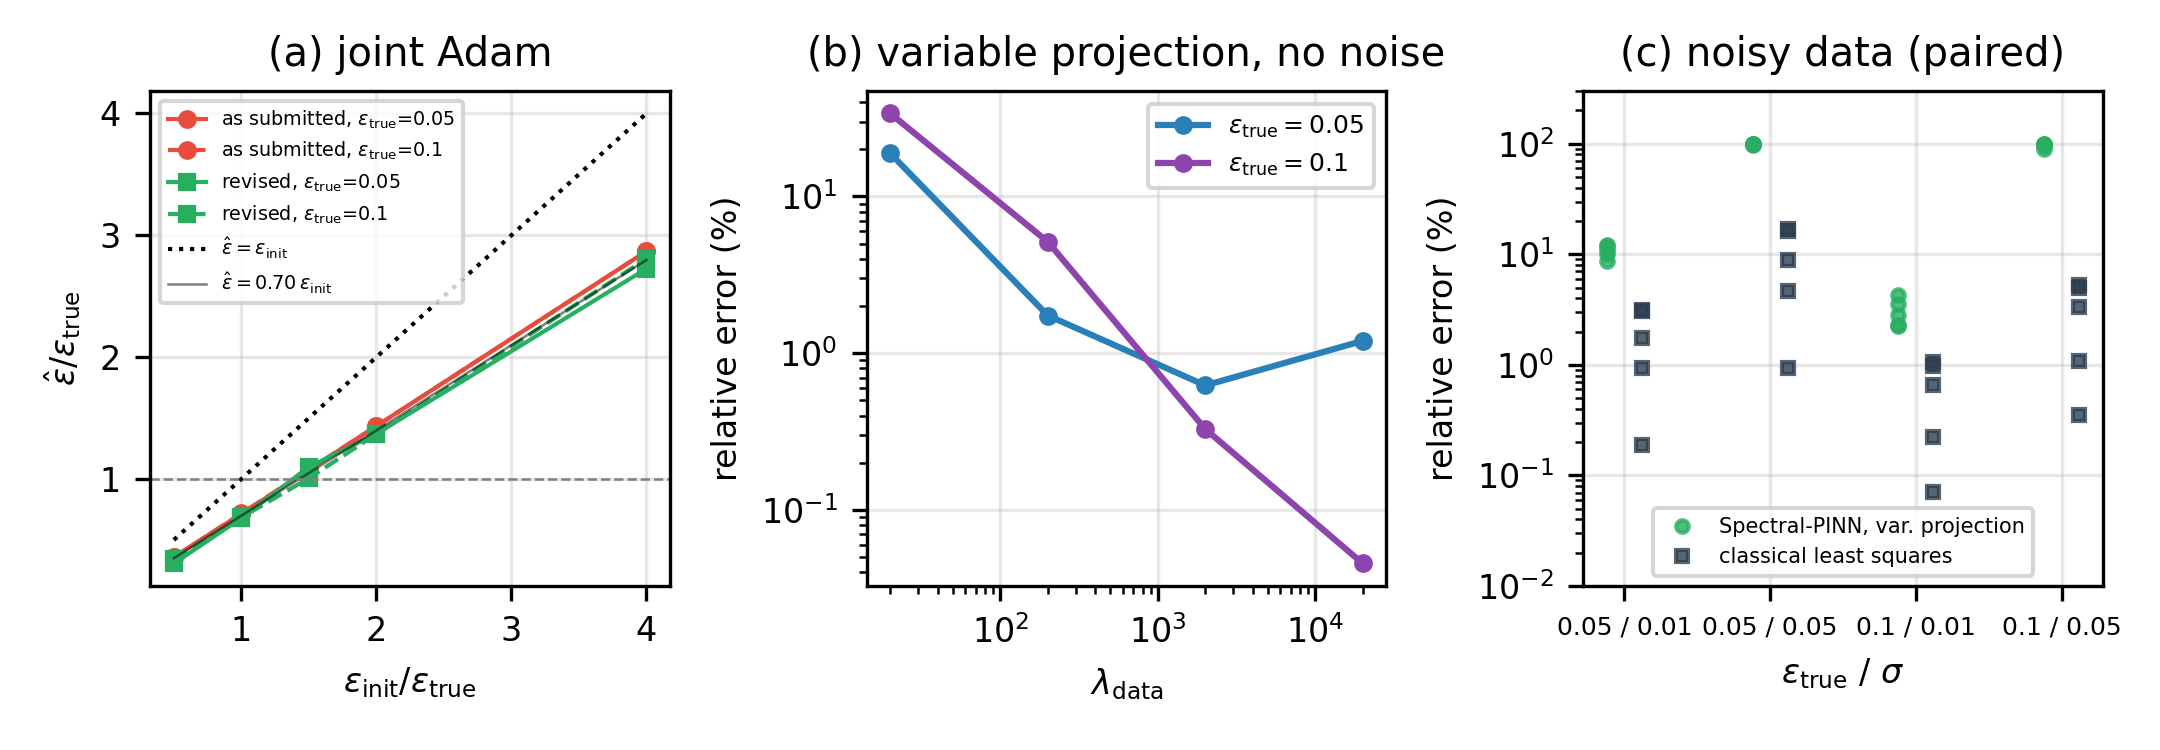
\includegraphics[width=\textwidth]{figures_r1/fig_inverse.png}
\caption{\rev{(a) Joint Adam: $\hat\varepsilon/\varepsilon_{\rm true}$ versus the starting value, for the as-submitted and the revised network. The estimate follows $\approx0.7\,\varepsilon_{\rm init}$ (dotted: no change; dashed: the true value). (b) Variable projection: relative error versus the data weight, noise-free data. (c) Noisy data: relative errors of the variable-projection Spectral-PINN and of classical least squares on the same five noise realizations (horizontal axis: $\varepsilon_{\rm true}$, upper row; $\sigma$, lower row).}\label{fig:inverse}}
\end{figure}

\subsubsection{Identifiability}

\rev{The data constrain $\varepsilon$ only through the term $\varepsilon^2u_{xx}$. This term is small on this benchmark. For our design (40 points, 5 times) the norm of the derivative of the data vector with respect to $\log\varepsilon$ is \N{ident.S001} at $\varepsilon=0.01$, \N{ident.S005} at $0.05$ and \N{ident.S01} at $0.1$.}

\rev{With noise $\sigma=0.01$ the Cram\'er--Rao standard error of $\log\hat\varepsilon$ is \N{ident.se001} at $\varepsilon=0.01$ and \N{ident.se005} at $0.05$. Classical least squares has a root-mean-square error of \N{ident.cl001} at $0.01$ and \N{ident.cl005} at $0.05$ (\N{ident.n_rep} noise realizations). This matches the bound. At $\varepsilon=0.01$ no unbiased estimator can do better than about \N{ident.se001} with such data. The noise experiments at $\varepsilon=0.01$ in the first version were therefore not meaningful. The variable-projection network has errors of \N{inv.vp001.n0} without noise and \N{inv.vp001.n0.01} with noise at $\varepsilon=0.01$.}

\subsection{Two-Dimensional Symmetry}\label{sec:2d-results}

\rev{The two-dimensional results are unchanged from the first version. No Neumann condition is involved. We corrected the statements about them.} Table~\ref{tab:2d} gives the symmetry violation $S(t)$. The Fourier-Spectral-PINN stays at round-off: $S\in[\N{s2d.fmin},\N{s2d.fmax}]$ for $t\in[0,1]$ \rev{(one run). By the parity of the basis, $S$ is zero in exact arithmetic. The value shown is the round-off of the evaluation grid (Appendix~\ref{app:sym}), not an effect of training.} The vanilla PINN has the same periodic encoding. Its $S$ increases monotonically in all five seeds. It grows by a factor \N{s2d.growth} between $t=0$ and $t=1$ (seeds: \N{s2d.growth_range}).

\rev{Larger mode counts and a sharper interface change nothing (Table~\ref{tab:stress-2d}). At $t=1$ the violation lies between \N{s2d.smin} and \N{s2d.smax} in all five configurations. This is round-off level. The RMS asymmetry $\sqrt S$ is at most \N{s2d.rms_max}, about three times the machine epsilon. The violation is about three times larger for $\varepsilon=0.1$ than for $\varepsilon=0.3$. Doubling $M$ or the budget does not change it. The first version gave the range as ``$10^{-31}$--$10^{-31.4}$''. This was inconsistent with its own table.}

% generated by make_tex_r1.py -- do not edit
\begin{table}[H]
\tablesize{\footnotesize}
\caption{Reflection-symmetry violation $S(t)$ (Section~\ref{sec:2d}) of the Fourier-Spectral-PINN (one run; $M=8$, $\varepsilon=0.3$) and of a vanilla PINN with the same periodic input encoding (mean~$\pm$~SD over five seeds). Data of the first version, unchanged.\label{tab:2d}}
\newcolumntype{C}{>{\centering\arraybackslash}X}
\begin{tabularx}{\textwidth}{cCC}
\toprule
\ensuremath{\boldsymbol{t}} & \textbf{Fourier-Spectral-PINN} & \textbf{Vanilla PINN (5 seeds)}\\
\midrule
0.0 & \ensuremath{8.7\times10^{-32}} & \ensuremath{(4.12\pm1.13)\times10^{-5}}\\
0.2 & \ensuremath{9.4\times10^{-32}} & \ensuremath{(4.94\pm1.16)\times10^{-5}}\\
0.5 & \ensuremath{1.0\times10^{-31}} & \ensuremath{(9.46\pm1.81)\times10^{-5}}\\
1.0 & \ensuremath{1.3\times10^{-31}} & \ensuremath{(2.22\pm0.45)\times10^{-4}}\\
\bottomrule
\end{tabularx}
\end{table}

\begin{table}[H]
\tablesize{\footnotesize}
\caption{Fourier-Spectral-PINN: reflection-symmetry violation at $t=1$ for larger mode numbers $M$ and a sharper interface ($\varepsilon=0.1$). $\sqrt{S}$ is the root-mean-square asymmetry, to be compared with the machine epsilon $2.2\times10^{-16}$.\label{tab:stress-2d}}
\newcolumntype{C}{>{\centering\arraybackslash}X}
\begin{tabularx}{\textwidth}{cCCCC}
\toprule
\ensuremath{\boldsymbol{M}} & \ensuremath{\boldsymbol{\varepsilon}} & \textbf{Epochs} & \ensuremath{\boldsymbol{S(1)}} & \ensuremath{\boldsymbol{\sqrt{S(1)}}}\\
\midrule
8 & 0.3 & 3000 & \ensuremath{1.27\times10^{-31}} & \ensuremath{3.6\times10^{-16}}\\
16 & 0.3 & 3000 & \ensuremath{1.27\times10^{-31}} & \ensuremath{3.6\times10^{-16}}\\
16 & 0.3 & 6000 & \ensuremath{1.26\times10^{-31}} & \ensuremath{3.5\times10^{-16}}\\
8 & 0.1 & 3000 & \ensuremath{3.74\times10^{-31}} & \ensuremath{6.1\times10^{-16}}\\
16 & 0.1 & 6000 & \ensuremath{3.74\times10^{-31}} & \ensuremath{6.1\times10^{-16}}\\
\bottomrule
\end{tabularx}
\end{table}

